\subsection{Dataset}

\begin{figure}[h]
    \centering
    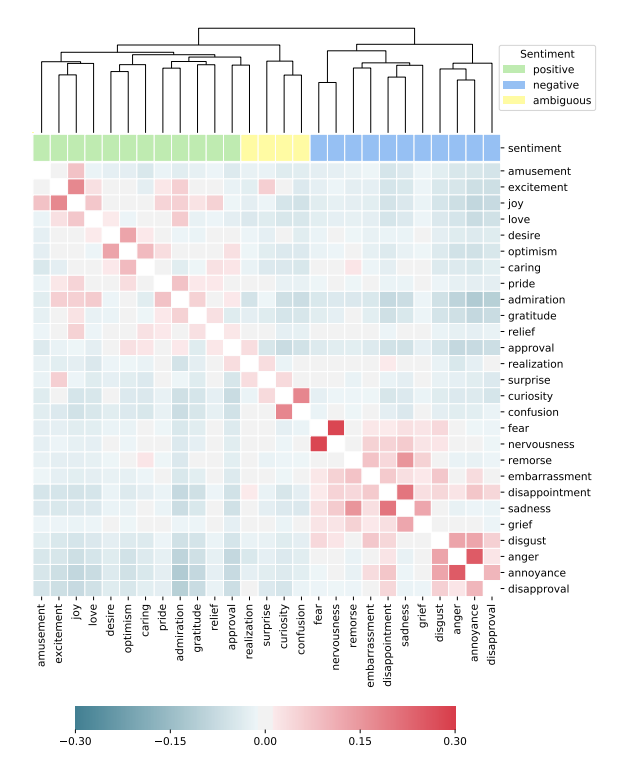
\includegraphics[width=8.4cm]{img/corr.png}
    \caption{Annotation results of the GoEmotions dataset. The heatmap shows the correlation between ratings for each emotion. The dendrogram represents the a hierarchical clustering of the ratings \citet{demszky2020goemotions}.}
\label{fig:corr}
\end{figure}


GoEmotions is a large dataset that consists of 58K English Reddit comments, each of which is labeled with one or more of 28 emotions (including ``neutral''). While GoEmotions characterizes a multi-label emotion classification task, most (83\%) of the samples have a single label. 


Despite some degree of inter-rater agreement, the heatmap from  Figure \ref{fig:corr} shows, some nuanced emotions, such as ``disgust'', ``anger'' ,and ``annoyance'' (bottom right corner), present even some annotation challenges. Such a fine-grained emotion taxonomy requires more a careful design of classifiers. 


\subsection{Model and Parameter}

To draw a fair comparison and demonstrate the benefit of label-aware attention, we use the same language model as \citet{demszky2020goemotions}, which is a pretrained cased \textsc{Bert Base}. The vector representation for each label is initialized to be a 768-dimensional word embedding of the corresponding emotion. However, the label representations are finetuned separately from the word embedding. Finally, the feedforward network in the classification head is a single linear layer with a bias term. 

When finetuning the pretrained \textsc{Bert} model, we use the same set of hyperparameters as \citet{demszky2020goemotions}. Specifically, the batch size is 16 and the learning rate is 5e-5 with the slanted triangular scheduler. For the CB loss, we choose $\beta = 0.95$. The finetuning is run for 4 epochs with no parameter held frozen. We run 10 experiments for each model under different seeds, and we average the performance over 10 experiments. 

\subsection{Results}\label{sec:res}
% \subsection{Model Statistics}
In Table \ref{tab:res}, we see that our model, which is equipped with label-aware attention (LAA) mechanism and trained under class-balanced (CB) loss, outperforms the baseline model. The Marco-average F1 of our model is 0.06 higher than that of the baseline model. Moreover, our model shows much lower variance under different seeds, which is an indication of robust design.


Aside from our best model, we also run two experiments which respectively involve LAA and LEAM only, and the results are presented in Appendix Table \ref{tab:full}. We see that our three models all outperform the baseline model, and the use of CB loss improved performance for the LAA model. 

\begin{table}[h]
    \begin{center}
    \begin{tabular}{|l |c| c|}
        \hline
         $\quad \quad \quad$ \textbf{Emotions} $\quad \quad \quad$ &  $\quad \quad \quad $ \textbf{Baseline}  $\quad \quad \quad $ & \textbf{LAA w/ CB Loss (ours)} \\ % &LEAM w/CE Loss\\
        \hline\hline
        Admiration &  0.65 & \textbf{0.67} \\
        Amusement & 0.80 & \textbf{0.81} \\
        Anger & 0.47 &\textbf{0.49} \\
        Annoyance & 0.34 &\textbf{0.37}\\
        Approval & 0.36 & \textbf{0.41}\\
        Caring & 0.39 & \textbf{0.43} \\
        Confusion & 0.37 &\textbf{0.42} \\
        Curiosity & 0.54 & \textbf{0.56}\\
        Desire & \textbf{0.49} & \textbf{0.49}\\
        Disappointment & 0.28 &\textbf{0.33} \\
        Disapproval & 0.39 & \textbf{0.41} \\
        Disgust & 0.45 & \textbf{0.48} \\
        Embarrassment & 0.43 &\textbf{0.45}\\
        Excitement & 0.34 & \textbf{0.41}\\
        Fear &  0.60 & \textbf{0.67} \\
        Gratitude & 0.86 & \textbf{0.90}\\
        Grief & 0.00 & \textbf{0.42}\\
        Joy & 0.51 & \textbf{0.60}\\
        Love & 0.78 & \textbf{0.79} \\
        Nervousness & \textbf{0.34} & \textbf{0.34} \\
        Neutral & \textbf{0.68} & 0.67\\
        Optimism & 0.51 & \textbf{0.56}\\
        Pride &  0.36 & 0.49\\
        Realization & 0.21 & \textbf{0.26}\\
        Relief & 0.15 & \textbf{0.36} \\
        Remorse & 0.66 & \textbf{0.68} \\
        Sadness & 0.49 & \textbf{0.53} \\
        Surprise & 0.50 & \textbf{0.54} \\
        \hline
        Macro Avg. & 0.46 &\textbf{0.52}\\
        \hline
        Std & 0.19 & 0.01 \\ % &\textbf{0.005} \\
        \hline
    \end{tabular}
    \end{center}
    \caption{F1 scores across all emotions in GoEmotions dataset, in comparison with baseline. Our method combines the Label-Aware Attention (LAA) with class-balanced (CB) cross-entropy loss.} % ; and LEAM model with cross entropy loss.}
    \label{tab:res}
\end{table}

%  Our model achieves significant improvement on Macro-average F1 and consistent improvements across all emotion groups. Moreover, the model shows much lower variance under different seeds, an indication of robust design.

\subsection{Error Analysis}

As discussed in table \ref{tab:res}, our methods outperform the baseline model. We see that our model performs better in almost all emotions compared to the baseline model. In the last report, we argued that the baseline model often fails to distinguish between ``neutral" and other emotions (see Appendix, table \ref{table:baseE}). In this section, we will examine qualitatively how our best-performing model (LAA with CB loss) is better than the baseline model. 

For the sake of simplicity, we use the following procedures in later error analysis. If the sample contains only has 1 true label, then it is considered correctly classified if the top 1 predicted label is the same as the true label. If the sample contains multiple true labels, it is considered correct if all its label is contained in the top 3 predicted label. 

\begin{table}[h!]
\centering
\begin{tabular}{l  l  c }
\hline\hline
True Label& Predicted Label & Occurrence  \\ [0.5ex]
\hline 
neutral  & amusement  & 50\\
neutral  & anger  & 36\\
neutral  & approval  & 32\\
neutral  & annoyance  & 23\\
neutral  & curiosity  & 16\\
curiosity   & anger  & 13\\
approval  &  anger  & 11\\
neutral &  admiration  & 11\\[1ex]
\hline 
\end{tabular}
\vspace{1ex}
\caption{Top 8 common circumstances where the text is misclassified by the baseline model but are correctly classified by our model}
\label{table:imp} 
\end{table}

Table \ref{table:imp} present the top 8 circumstances where the text is misclassified by the baseline model but are correctly classified by our model. We see that our model effectively prevents ``neutral" from being misclassified as other emotions. However, there is little improvement in preventing other emotions from being misclassified as ``neutral". 

\begin{table}[h!]
\centering
\begin{tabular}{l  l  l l l} \hline \hline 
ID &Sentence & True Label& Predicted Label  \\ [0.5ex]
\hline
(A)& Everyone knows the good [NAME] are the dirty little devil's & neutral  & annoyance\\[1ex]
(B) &[NAME]? never met one those. & neutral  & curiosity\\[1ex]
\hline 
\end{tabular}
\vspace{1ex}
\caption{Two representative mistakes of the baseline model, correctly classified by our model}
\label{table:exp} 
\end{table}

Table \ref{table:exp} presents two representative sentences that are misclassifed by the baseline model but are correctly classified by our model. We see that the two sentences both employ rhetoric techniques that would make them liable to being misclassified for models that do not fully understand the semantics but instead rely on certain features of the sentence to make the classification (e.g., ``?" in text (B)). The fact that they are correctly classified by our model suggests that the label-aware attention mechanism effectively facilitated natural language understanding (NLU) in our model. 


